\documentclass[10pt,]{beamer}

\usepackage{pgfpages}
\usepackage[style=authortitle,backend=bibtex]{biblatex}
\bibliography{Bibliography}
\addbibresource{Bibliography.bib}

\mode<handout>{%
    \pgfpagesuselayout{4 on 1}[a4paper,landscape] 
    %\setbeameroption{show notes}
    \setbeamercolor{note page}{bg=white}
}

\usepackage[]{amsmath}
\usepackage{amsthm,amssymb,amsfonts}
\usepackage{graphicx,xfrac,mathrsfs,subcaption}
\usepackage{tikz,pgfplots}
\usepackage{tikzpagenodes}
\usepackage{multicol,multirow}

\usetikzlibrary{positioning,automata}
\usetikzlibrary{matrix}
\usetikzlibrary{arrows,shapes}
\usetikzlibrary{trees}
\usetikzlibrary{backgrounds}
\usetikzlibrary{shapes.geometric}
\usetikzlibrary{calc,shapes.callouts,shapes.arrows}
\usetikzlibrary{graphs}
\usetikzlibrary{positioning, arrows}
\usetikzlibrary{fit}

\tikzset{onslide/.code args={<#1>#2}{%
  \only<#1>{\pgfkeysalso{#2}}
}}


%%%%%%%%%%%%%%%%%%%%%%%%%%%%
%%%%%%%%%%%%%%%%%%%%%%%%%%%%
%%%%% long and short versions
\newcommand{\extra}[1]{}
\newcommand{\short}[1]{#1}

% \usetheme{Warsaw}
\definecolor{faded}{HTML}{8693AB}
\makeatletter
\def\th@mystyle{%
    \normalfont % body font
    \setbeamercolor{block title example}{bg=faded,fg=white}
    \setbeamercolor{block body example}{bg=faded!20,fg=black}
    \def\inserttheoremblockenv{exampleblock}
  }
\makeatother
\theoremstyle{mystyle}
\newtheorem*{conjecture}{Conjecture}

\usetheme{Boadilla}
\makeatother
\setbeamertemplate{footline}
{
	\leavevmode%
	\hbox{%
	\begin{beamercolorbox}[wd=.4\paperwidth,ht=2.25ex,dp=1ex,center]{author in head/foot}%
		\usebeamerfont{author in head/foot}\insertshortauthor
	\end{beamercolorbox}%
	\begin{beamercolorbox}[wd=.6\paperwidth,ht=2.25ex,dp=1ex,center]{title in head/foot}%
		\usebeamerfont{title in head/foot}\insertshorttitle\hspace*{3em}
		\insertframenumber{} / \inserttotalframenumber\hspace*{1ex}
	\end{beamercolorbox}}%
	\vskip0pt%
}
\makeatletter

\setbeamertemplate{navigation symbols}{}
\title[HK-property | Perfect Binary Trees]{Exploring perfect binary trees with relation to the HK-property}
\subtitle{MXML Presentation} %This is where you can specify the conference name or presentation venue
\author[A.M, M.N.S]{Atishaya Maharjan \\ Mahsa N. Shirazi}
\date{\today}

\begin{document}
\parskip = \baselineskip

\begin{frame} %Title page
    \titlepage
\end{frame}

\begin{frame}{Outline}
    \tableofcontents
\end{frame}

\begin{frame}
    \frametitle{Introduction}
    \begin{itemize}
        \item Providing an overview of the Erdős-Ko-Rado (EKR) theorem and its relevance to intersecting families of sets.
        \item Introducing perfect binary trees and their relation to the HK-property.
        \item Objectives of this presentation:
              \begin{itemize}
                  \item Exploring properties of perfect binary trees.
                  \item Discussing the HK-property.
                  \item Investigating potential connections between perfect binary trees and the HK-property.
              \end{itemize}
    \end{itemize}
\end{frame}

\begin{frame}\frametitle{EKR Theorem}
    \begin{itemize}
        \item \footcite{Erds1961INTERSECTIONTF} The Erdős-Ko-Rado (EKR) theorem, named after mathematicians Paul Erdős, Chao Ko, and Richard Rado, is a fundamental result in extremal set theory.
        \item The theorem deals with intersecting families of sets, which are collections of sets that share a common non-empty intersection.
        \item  Specifically, the EKR theorem provides conditions under which the size of the largest intersecting family of sets can be determined.
        \item \footcite{MR0892525} This result has applications in combinatorics, graph theory, probability and other areas of statistics and mathematics.
    \end{itemize}
\end{frame}

\section{EKR Theorem}
\begin{frame}\frametitle{EKR Theorem}
    \begin{definition}[Intersecting family]
        A family of subsets $\mathcal{F}$ of some set is \textbf{intersecting} if any two members of $\mathcal{F}$ have a non-empty intersection.
    \end{definition}
    \begin{itemize}
        \item The \textbf{Erd\H{o}s-Ko-Rado}  theorem limits the number of sets in an intersecting family.
    \end{itemize}
    \begin{theorem}[EKR Theorem]
        \footcite{Godsil_Meagher_2015} If $\mathcal{F}$ is an intersecting family of $k$-subsets of an $n$-set (cardinality of the set is $n$), then
        \begin{itemize}
            \item $|\mathcal{F}| \leq \binom{n - 1}{k - 1}$
            \item If equality holds, $\mathcal{F}$ consists of the $k$-subsets that contain $i$, for some $i$ in the $n$-set.
        \end{itemize}
    \end{theorem}
\end{frame}

\section{HK-property}
\begin{frame}\frametitle{HK-property}
    Some definitions before we get into the property:

    \begin{definition}[Cocliques]
        \begin{itemize}
            \item A \textbf{coclique} in a graph is a set of vertices such that no two vertices in the set are adjacent.
            \item The maximum size of a coclique in a graph is called the \textbf{indepdence number} of the graph. For a graph $G$, it is denoted by $\alpha(G)$.
        \end{itemize}
    \end{definition}

    \begin{definition}[Stars and Stars Center]
        \begin{itemize}
            \item Let $G = (V, E)$ be a graph, and $v \in V(G)$. The family $\mathcal{I}^k_G(v) = {A \in \mathcal{I}^k_G : v \in A}$ is called a \textbf{star} of $\mathcal{I}^k_G$ and $v$ is called it's \textbf{star center}.
        \end{itemize}
    \end{definition}

    \begin{definition}[k-EKR graph]
        A graph is said to be $k$-EKR if for any family of indepdent sets $\mathcal{I}^k_G$ of size $k$, the intersection of any two sets in $\mathcal{I}^k_G$ is non-empty and that $|\mathcal{F}| \leq \mathcal{I}^k_G(v)$, for a vertex $v \in V(G)$.
    \end{definition}
\end{frame}

\begin{frame}\frametitle{HK-property}
    Studying the EKR theorem, \footcite{HOLROYD2005165} Holroyd and Talbot made the following two conjectures:
    \begin{conjecture}[k-EKR Conjecture]
        Let $G$ be a graph, and let $\mu(G)$ be the size of its smallest maximal independent set. Then $G$ is $k$-EKR for every $1 \leq k \leq \frac{\mu(G)}{2}$.
    \end{conjecture}
    \begin{conjecture}[HK-Property]
        For any $k \geq 1$ and any tree $T$, there exists a leaf $l$ of $T$ such that $|\mathcal{I}^k_T(v)| \leq |\mathcal{I}^k_T(l)|$ for each $v \in V(T)$.
    \end{conjecture}
\end{frame}

\begin{frame}\frametitle{HK-property}
    \begin{itemize}
        \item The HK-property was proven for $k \leq 4$, but the conjecture was shown to be false.\footcite{MR2523796} \footcite{MR3612439} \footcite{MR3271819}
    \end{itemize}

    \begin{figure}
        \centering
        \begin{tikzpicture}[scale=0.7,level distance=2cm,
                level 1/.style={sibling distance=8cm},
                level 2/.style={sibling distance=4cm},
                level 3/.style={sibling distance=2cm},
                every node/.style={circle, draw, fill=white, minimum size=1.75em},]
            \node (v11) {$v_0$}
            child {node (v21) {$v_1$}
                    child {node  {}
                            child {node {}}
                        }
                    child {node (v32) {}
                            child {node {}}
                        }
                }
            child {node (v22) {$v_2$}
                    child {node (v33) {}
                            child {node {}}
                        }
                    child {node (v34) {}
                            child {node {}}
                        }
                };
        \end{tikzpicture}
        \caption*{The largest k-star for $k \geq 5$ is centered at $v_0$}
    \end{figure}
\end{frame}

\begin{frame}\frametitle{Some graphs that DO satisfy the HK-property}
    \footcite{MR4245360} The HK-property holds for spiders, caterpillars, and (partially) lobsters.
    <INSERT IMAGES HERE WHEN YOU HAVE TIME>
\end{frame}

\section{Perfect Binary Trees}
\begin{frame}\frametitle{Perfect Binary Tree}
    \begin{definition}[Depth of a vertex]
        For a tree $T = (V, E)$ with a root vertex $r \in V$, the \textbf{depth} of a vertex $v \in V$ is defined as the length of the path from the $r$ to $v$.
    \end{definition}
    \begin{definition}[Binary Tree]
        A \textbf{binary tree} is a tree in which each vertex has at most two children, referred to as the left child and the right child.
    \end{definition}
    \begin{definition}[Perfect Binary Tree]
        A \textbf{perfect binary tree} is a binary tree in which all the internal nodes have exactly two children and all the leaves are at the same depth.
    \end{definition}
\end{frame}

\begin{frame}\frametitle{Perfect Binary Tree}
    \begin{definition}
        Let $\mathcal{V}_k \in V(T)$ be the set of vertices of depth $k$. We call $\mathcal{V}_k$ as the depth vertex set of depth $k$. Index all vertices in $\mathcal{V}_k$ from left to right as $v_{k, i}$, where $k$ is the depth of the vertex and $i$ is the index of the vertex in $\mathcal{V}_k$ such that $1 \leq i \leq 2^{k - 1}$.
    \end{definition}
    \begin{figure}
        \centering
        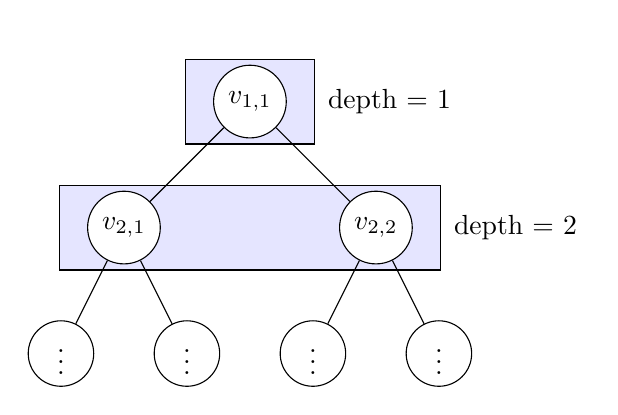
\begin{tikzpicture}[scale=0.4,level distance=4cm,
                level 1/.style={sibling distance=8cm},
                level 2/.style={sibling distance=4cm},
                level 3/.style={sibling distance=2cm},
                every node/.style={circle, draw, fill=white}]
            \node (v11) {$v_{1,1}$}
            child {node (v21) {$v_{2,1}$}
                    child {node {$\vdots$}}
                    child {node {$\vdots$}}
                }
            child {node (v22) {$v_{2,2}$}
                    child {node {$\vdots$}}
                    child {node {$\vdots$}}
                };

            \begin{scope}[on background layer]
                \node[draw,rectangle,fit=(v11),inner xsep=10pt, inner ysep=2pt, fill=blue!10, label=right:{depth = 1}] {};
                \node[draw,rectangle,fit=(v21) (v22),inner xsep=10pt, inner ysep=2pt, fill=blue!10, label=right:{depth = 2}] {};
            \end{scope}
        \end{tikzpicture}
    \end{figure}
\end{frame}


%%%%%%%%%%%%%%%%%%%%%%%%%%%%%%%%%%%%%%%%%%%%%%%%%%%%%%%%%%%%%%%%%%%%%%
%%%%%%%%%%%%%%%%%%%%%%%%%%%%%%%%%%%%%%%%%%%%%%%%%%%%%%%%%%%%%%%%%%%%%%  
%%%%%%%%%%%%%%%%%%%%%%%%%%%%%%%%%%%%%%%%%%%%%%%%%%%%%%%%%%%%%%%%%%%%%%
\begin{frame}\frametitle{Thank You!}
    \framesubtitle{Summary}
    A slideshow usually ends with a summary slide.
\end{frame}




%%%%%%%%%%%%%%%%%%%%%%%%%%%%%%%%%%%%%%%%%%%%%%%%%%%%%%%%%%%%%%%%%%%%%%
%%%%%%%%%%%%%%%%%%%%%%%%%%%%%%%%%%%%%%%%%%%%%%%%%%%%%%%%%%%%%%%%%%%%%%  
%%%%%%%%%%%%%%%%%%%%%%%%%%%%%%%%%%%%%%%%%%%%%%%%%%%%%%%%%%%%%%%%%%%%%%

\end{document}